\chapter{EVALUATION}
\par Describe the evaluation process here. Take a maximum of 10 pages.
\section{Analysis I}
\par This is how to refer to a table using \emph{label} and \emph{ref}. The results are given in Table \ref{tab:largescale}

\begin{table}[ht]
    \centering
    \begin{tabular}{|p{2.5cm}|p{3cm}|p{3cm}|p{3cm}|}
        \hline
        Test Suite Size & SMM\footnote{Single Machine Model} & DM without SS\footnote{Distributed Model without State Saving} & Proposed Method \\
        \hline
        4 IP / 5 TC & 3.12 mnt & 1.04 mnt & 44.87 sec \\
        \hline
        41 IP/ 5 TC & 25.45 mnt & 8.48 mnt & 2.71 mnt \\
        \hline
        41 IP/ 100 TC & 8.48 hr & 2.83 hr & 59.54 mnt \\
        \hline
    \end{tabular}
    \caption{Performance Analysis - I}
    \label{tab:largescale}
\end{table}

\par The measurements were taken with the automatic result aggregation module turned off. Thus the execution time stated above is of purely execution only. The time required for the selection of test cases and the comparison of results are not included in this measurements. This is because in each of the existing methods, similar analysis is needed and the time required is almost same for all the methods.
\vfill

\section{Analysis II}
\par This is how you refer to a figure. The graphical representation is given in Figure \ref{fig:graph}. All the measurements are in \emph{seconds} calculated with a nanosecond precision.

\begin{figure}[h]
    \centering
    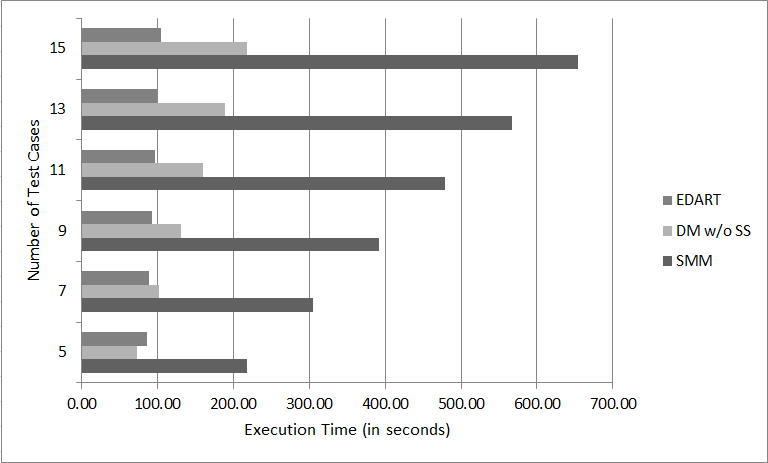
\includegraphics[width=\textwidth]{images/graph.png}
    \caption{Performance Comparison with Existing Systems}
    \label{fig:graph}
\end{figure}
\vfill

\newpage
